\documentclass{Fabiano_file}
\usepackage[table,usenames,dvipsnames]{xcolor}
\usepackage{tikz} %para desenhar
\usepackage{epstopdf}
\usepackage{hhline}
\usepackage{amsmath}
\usepackage{array}
\usepackage{cancel}
\usepackage{multirow}
\usepackage{bm}
\usepackage{float}
\usepackage{makecell} % diagonal table cells
\usepackage{tabularx}
\usepackage{bold-extra} % mini caps e negrito ao mesmo tempo %
\usepackage{fixltx2e} 
\usepackage{graphicx,amssymb}
\usepackage{subcaption} 
\usepackage{alltt}
\usepackage{mathtools}
\usepackage[figuresleft]{rotating}
\usepackage{caption}
\usepackage{varwidth}
\usepackage{longtable}

\usepackage[american,cuteinductors,smartlabels]{circuitikz}
\usepackage[hidelinks]{hyperref}
\usepackage[nottoc]{tocbibind}
\usepackage[a4paper,left=2cm,right=2cm,top=2cm,bottom=3cm]{geometry}

\usepackage[export]{adjustbox}
\usepackage{graphics}
\usepackage{amssymb, amsmath, amsthm}
\usepackage{float}

\usepackage{graphicx} 
\graphicspath{{Pictures/}} 
\usepackage{eso-pic}

\setcounter{secnumdepth}{5}


\usepackage{hyperref}
\hypersetup{
    colorlinks=true, %set true if you want colored links
    linktoc=all,     %set to all if you want both sections and subsections linked
    linkcolor=blue,  %choose some color if you want links to stand out
}

\usepackage{listings}
\usepackage{color}

\usepackage[pages=some,placement=centering]{background}

\lstdefinelanguage
   [x64]{Assembler}
   [x86masm]{Assembler}
   % add a "x64" dialect of Assembler
   % based on the "x86masm" dialect
   % with these extra keywords:
   {morekeywords={CJNE,JB,C,A,B,RI,MOVX, %
                  @,DPTR,MOVC,JNB,R0,R1,R2, %
                  R3,R4,R5,R6,R7,DJNZ,CLR,SETB,LCALL,SJMP,RETI,RET,CPL,TH1,TL1,ET1}} 

\definecolor{mygreen}{rgb}{0,0.6,0}
\definecolor{mygray}{rgb}{0.5,0.5,0.5}
\definecolor{mymauve}{rgb}{0.58,0,0.82}
\lstset{ %
  backgroundcolor=\color{gray},   % choose the background color; you must add \usepackage{color} or \usepackage{xcolor}
  basicstyle=\footnotesize,        % the size of the fonts that are used for the code
  breakatwhitespace=false,         % sets if automatic breaks should only happen at whitespace
  breaklines=true,                 % sets automatic line breaking
  captionpos=b,                    % sets the caption-position to bottom
  commentstyle=\color{mygreen},    % comment style
  deletekeywords={...},            % if you want to delete keywords from the given language
  escapeinside={\%*}{*)},          % if you want to add LaTeX within your code
  extendedchars=true,              % lets you use non-ASCII characters; for 8-bits encodings only, does not work with UTF-8
  frame=single,	                   % adds a frame around the code
  keepspaces=true,                 % keeps spaces in text, useful for keeping indentation of code (possibly needs columns=flexible)
  keywordstyle=\color{blue},       % keyword style
  language={[x64]{Assembler}},                 % the language of the code
  otherkeywords={*,...},           % if you want to add more keywords to the set
  numbers=left,                    % where to put the line-numbers; possible values are (none, left, right)
  numbersep=5pt,                   % how far the line-numbers are from the code
  numberstyle=\tiny\color{mygray}, % the style that is used for the line-numbers
  rulecolor=\color{gray},         % if not set, the frame-color may be changed on line-breaks within not-black text (e.g. comments (green here))
  showspaces=false,                % show spaces everywhere adding particular underscores; it overrides 'showstringspaces'
  showstringspaces=false,          % underline spaces within strings only
  showtabs=false,                  % show tabs within strings adding particular underscores
  stepnumber=2,                    % the step between two line-numbers. If it's 1, each line will be numbered
  stringstyle=\color{red},     % string literal style
  tabsize=2,	                   % sets default tabsize to 2 spaces
  title=\lstname % show the filename of files included with \lstinputlisting; also try caption instead of title
}


\title{Projeto de Dispositivos Decodificados Utilizando o Microcontrolador 80c51}
\author{Aluno: Fabiano Aparecido Marino \\NºUsp:7143980}

\begin{document}

\backgroundsetup{contents={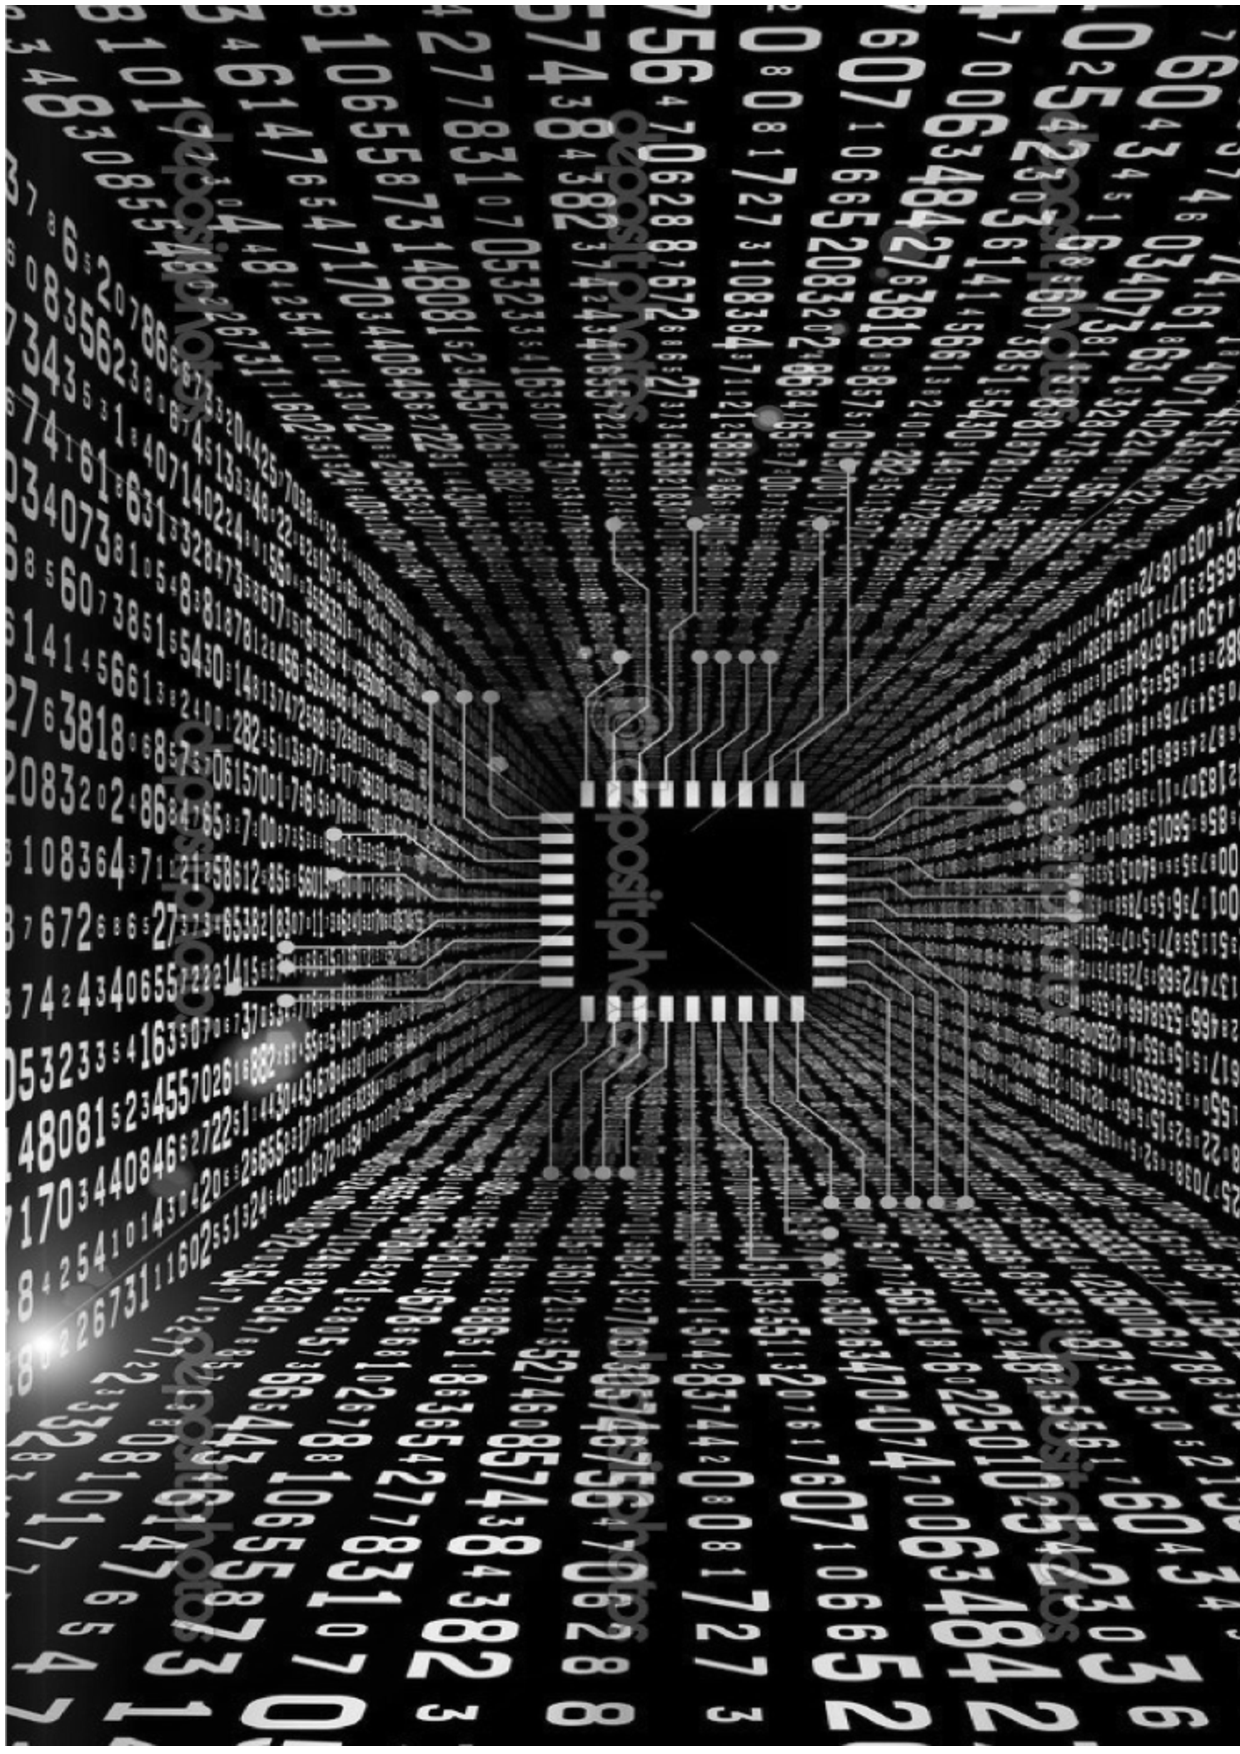
\includegraphics[width=70pt,height=90pt]{fundo1}},
		opacity=.1,
		angle={0}}

\BgThispage

\maketitle

\begin{figure}[h!]
\centering
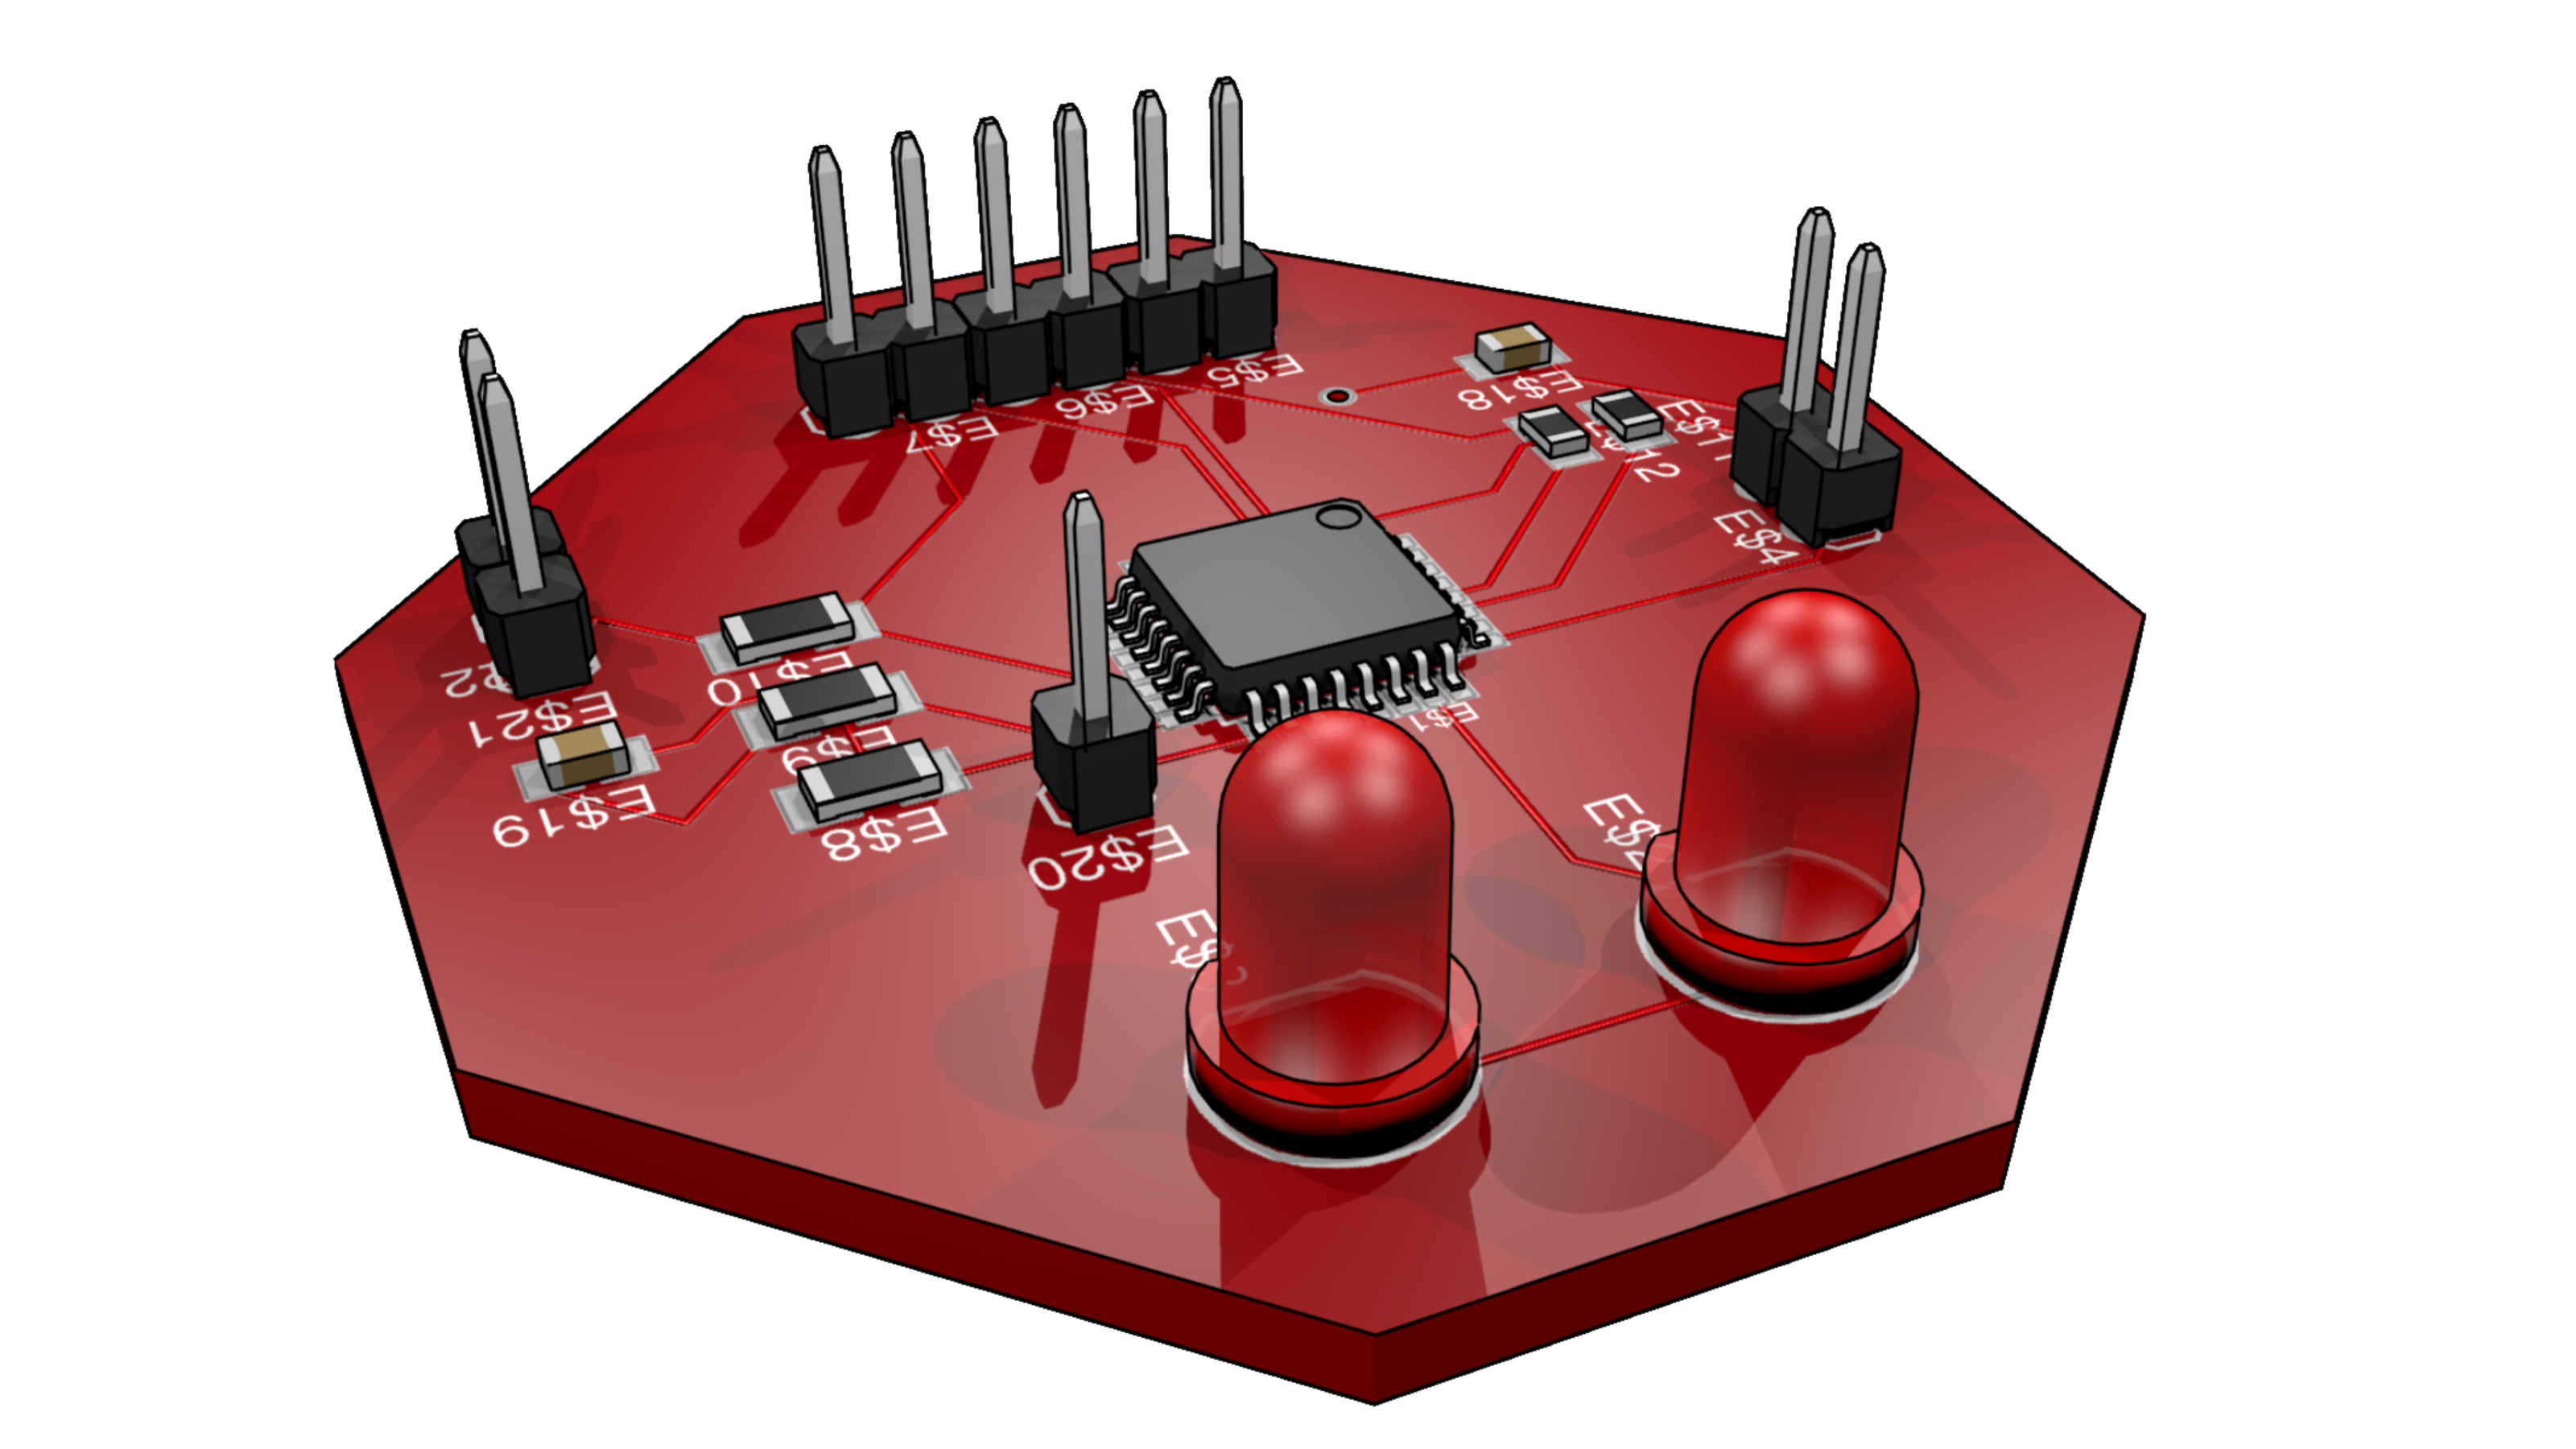
\includegraphics[width=1\textwidth]{example1.pdf}
\label{fig:adc_8051_dac_ideal}
\end{figure}


\newpage

Uma das características do microcontrolador 80c51 que o faz diferenciado é a possibilidade de se construir um hardware com disposistivos decodificados e fazer
o envio de um dado para um devido dispositivo de forma que o endereço em que o mesmo está decodificado possibilite o envio do dado ao dispositivo. Isto é possível
devido ao compartilhamento da porta \textit{P0} e \textit{P2} sendo que a P0 envia os dados e junção das portas possibilita o endereçamento do ponteiro DPTR.\\
O objetivo do seguinte projeto é contruir um hardware com o 80c51 de forma que contenha os seguintes periféricos:\\
\begin{itemize}
 \item Conversor ADC \textit{Analog to Digital Converter}.
 \item Conver DAC \textit{Digital to Analog Converter}.
 \item RS232 Terminal.
 \item Memória Ram de 8k.
 \item Memória Rom de 8k.
 \item Entrada Para Contador ou interrupção, podendo ser programada para ler um optoacoplador ou dispositivos dessa natureza.
 \item Teclado de Dezessei Botões.
 \\
\end{itemize}
 Abaixo encontrase a descrição, breve, de cada componente e o endereço que o mesmo ocupa.
 \begin{itemize}
 \item \textit{Memória Ram 6264 0000h--1fffh} : Trata-se de uma memória volatil de capacidade de armazenamento de 8kbytes. O datasheet da mesma encontra-se no seguinte endereço:
 \url{http://users.ece.utexas.edu/~valvano/Datasheets/6264.pdf}.
 
 \item \textit{Memória Rom 2764 2000h--3fffh} : Trata-se de uma memória não volatil de 8kbytes de armazenamento que pode ser utilizada nos projetos caso se necessite de mais memória
 do que os 4kbytes que o 80c51 oferece. O datasheet do componente pode ser encontrado com no seguinte endereço : \url{http://www.futurlec.com/Memory/2764_Datasheet.shtml}
 
 \item \textit{Conversor ADC0808 8000h--9fffh} : Trata-se do componente resnsável por possibilitar a conversão de analógica para digital possibilitando assim o processamento dos 
 dados provindos de meios externos a placa na forma analógica. O datasheet do componente encontra-se no seguinte endereço : \url{http://pdf.datasheetcatalog.com/datasheet/nationalsemiconductor/DS005687.PDF}
 
 \item \textit{Conversor DAC0808 6000h--7fffh} : Trata-se do componente responsável por fazer a conversão dos dados processados para sua forma analógica para que possam ser utilizados
 em atuadores oque inclui uma diversidade de possibilidades. O datasheet do componente encontra-se no seguinte endereço : \url{http://www.learn-c.com/adc0809.pdf}

 \item \textit{Latch 74hc373} : Trata-se do dispositivo reponsável por fazer a demultiplexação entre duto e dados e endereço do das portas p2 e p0 do micro 80c51.
 \url{http://www.nxp.com/documents/data_sheet/74HC_HCT373.pdf}
 
 \item \textit{74ls138} : Trata-se do dispositivo reponsável por decodificar cada elemento periférico que recebera ou enviara ao micro informações referente ao
 duto de dados. O datasheet do componente encontra-se no seguinte endereço : \url{http://pdf.datasheetcatalog.com/datasheets/90/232315_DS.pdf}
 
 \item \textit{Display LM016} : Dispositivo que possibilita a comunicação com o usuário visualmente.Trata-se de um display de duas linhas e dezesseis colunas.
 
 \item \textit{Teclado de Cristal Liquido 4000h--5fffh} Possibilita ao usuário que entre com valores que posteriormente serão processados pelo micro.
 
 \item \textit{Comunicação serial padrão RS232} Possibilita a comunicação com o usuário via interface serial.
 
 \item \textit{Fonte de Alimentação com tensões de fornecimento de +5, -5, +15, -15V}
 
 \item \textit{Driver de motor de passo} A placa acompanha um driver para controle de um motor de passo, sendo o mesmo constituido de um controlador l297 e um
 dispositivo de potência, o l298, pronto para ser usado na placa microprocessada.
 \end{itemize}
 
 Na Próxima pagina encontra-se o esquemático que corresponde ao projeto em questão.O mesmo foi criado e simulado no software proteus ISIS e sua confecção se deu 
 na Plataforma Ares.
 
  
 	\newpage
	%\thispagestyle{empty}
	\clearpage
	\begin{sidewaysfigure}
		\centering
		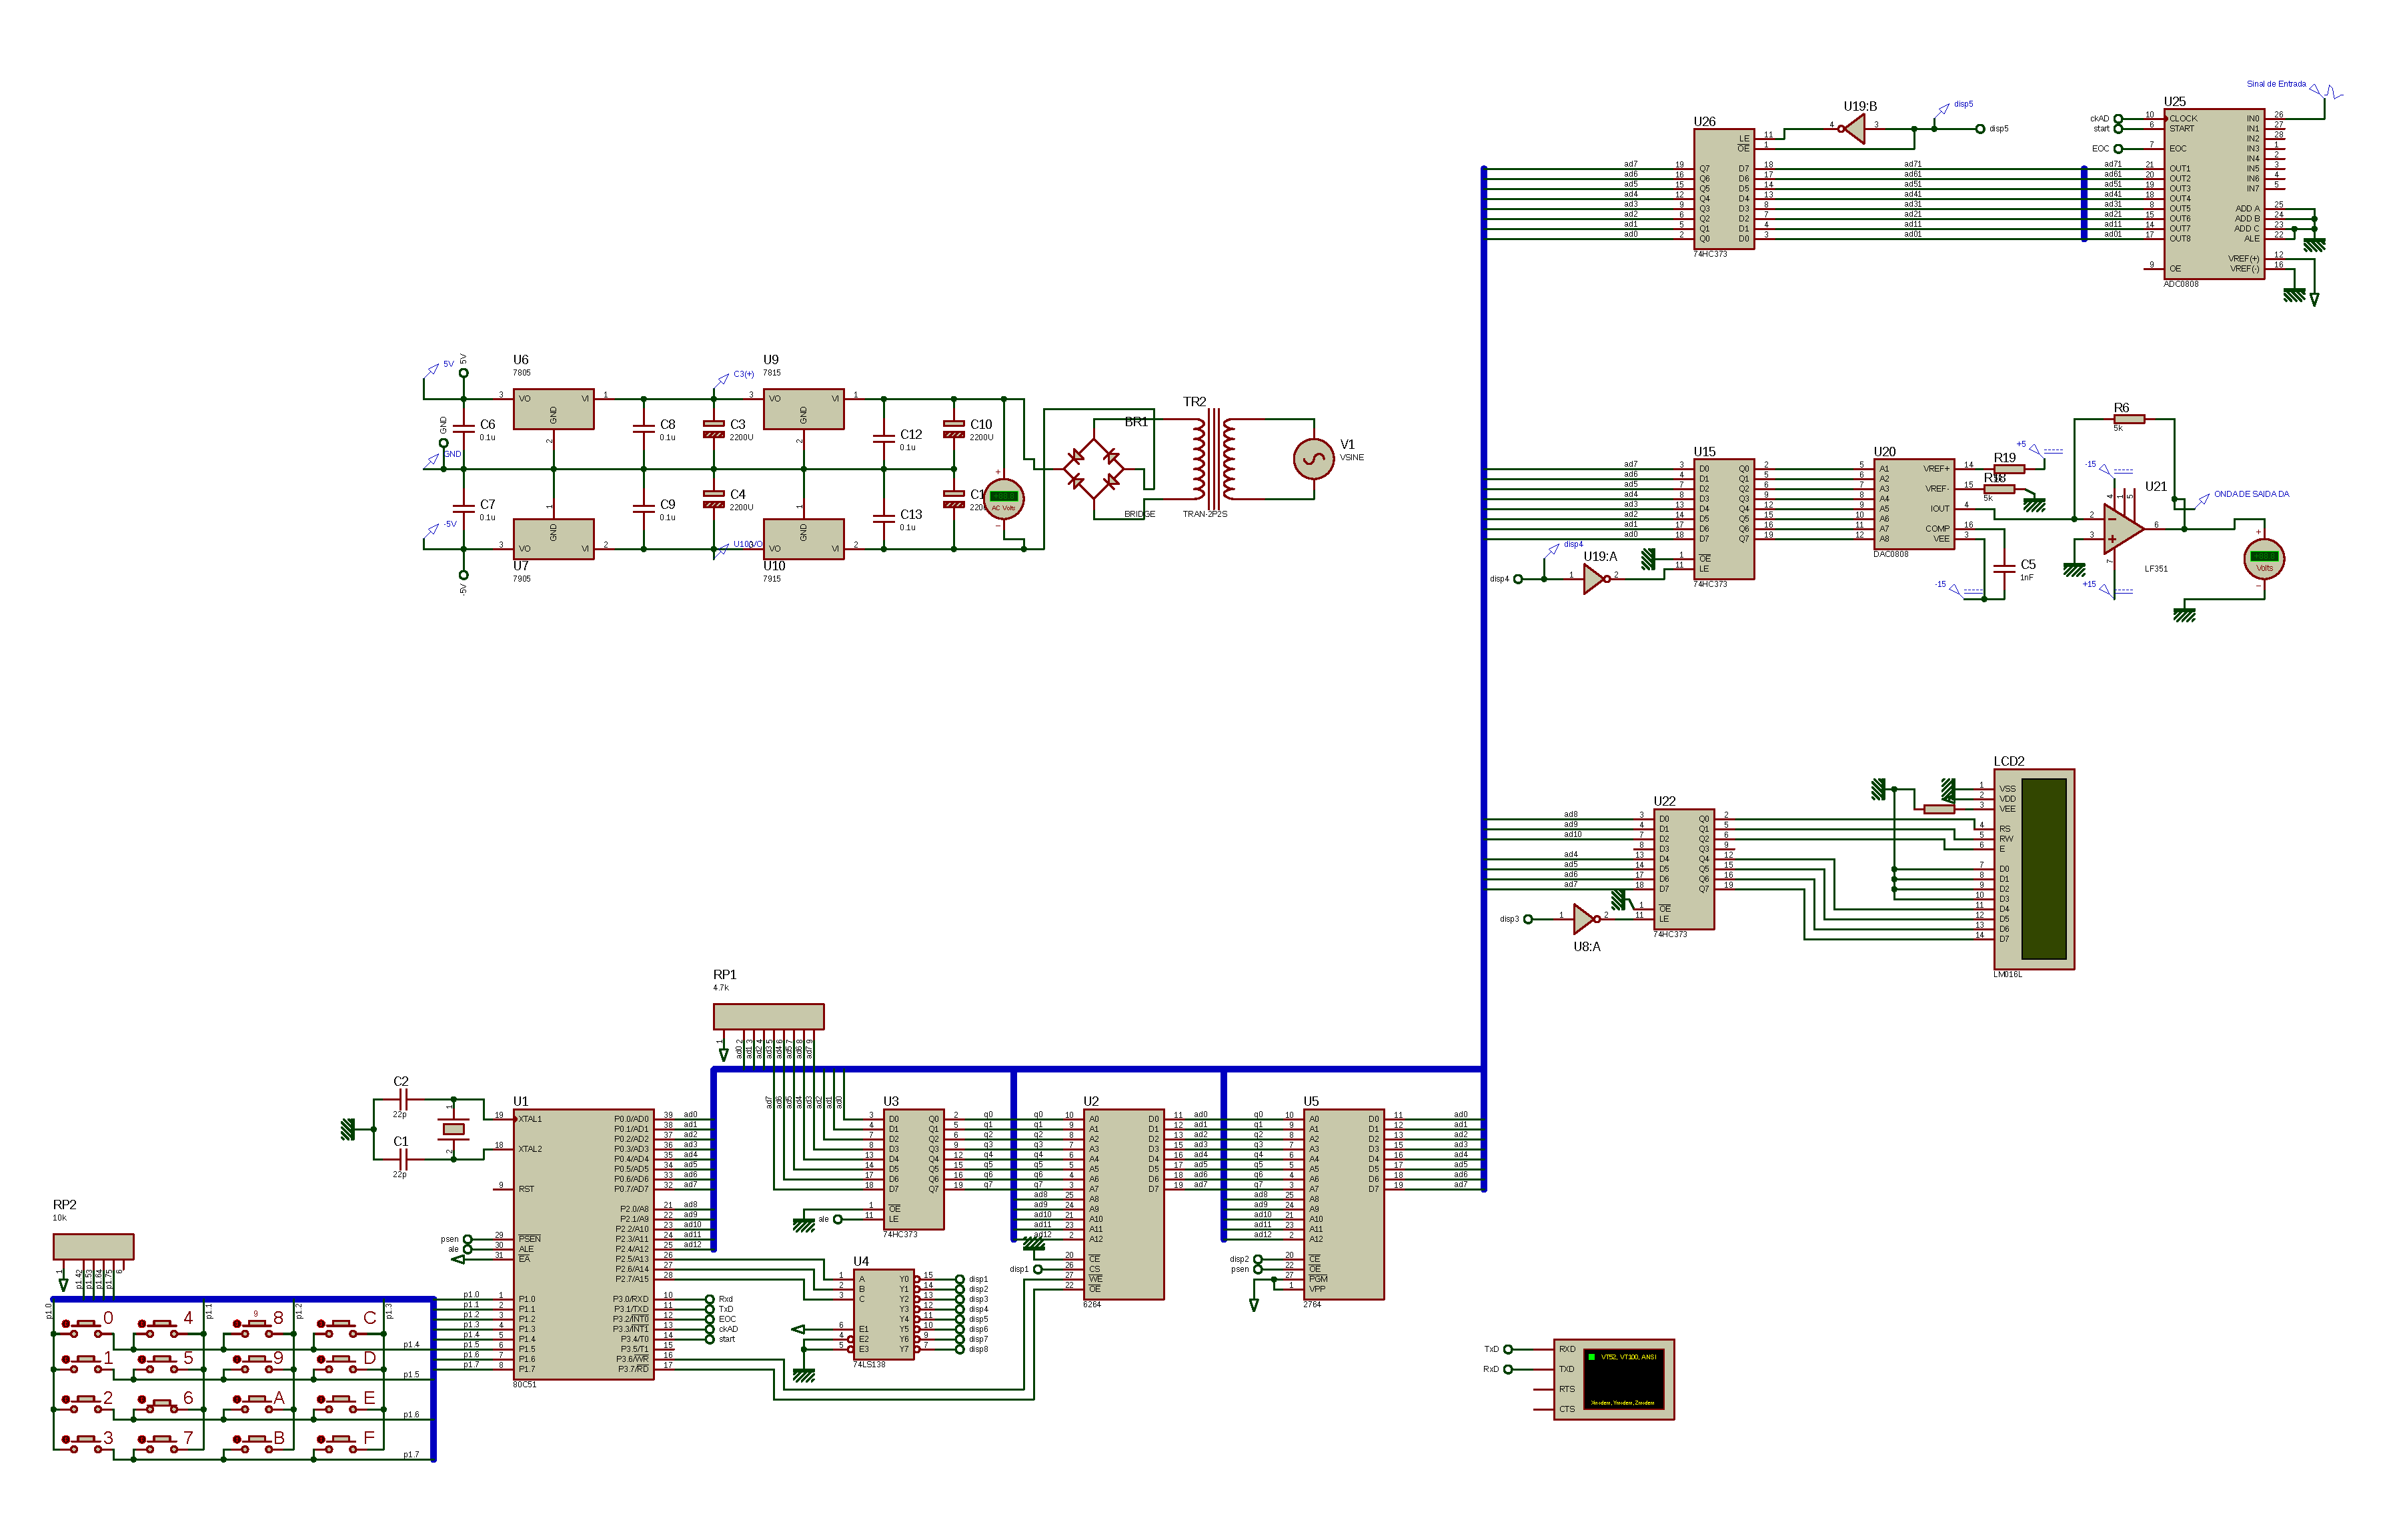
\includegraphics[width=1\linewidth]{projeto_dispositivos_decodificados}
		\label{fig:adc_dac_ideal}
	\end{sidewaysfigure}
	%\clearpage
	%\pagenumbering{gobble}
	\newpage


\section{Simulações de todas as possibilidades de caminho dos dados no barramentos e periféricos}
As imagens abaixo mostram as simulações da memória ram, conversor AD e DA e display de sete segmentos.O programa para simulação dos periféricos iterativos, como
teclado matricial e terminal serial ficam disponíveis no apêndice.

\begin{figure}[h!]
\centering
\includegraphics[width=.6\textwidth]{ad_da.pdf}
\caption{Simulação Conversores AD DA e 80c51}
\label{fig:adc_8051_dac_ideal}
\end{figure}

\begin{figure}[h!]
\centering
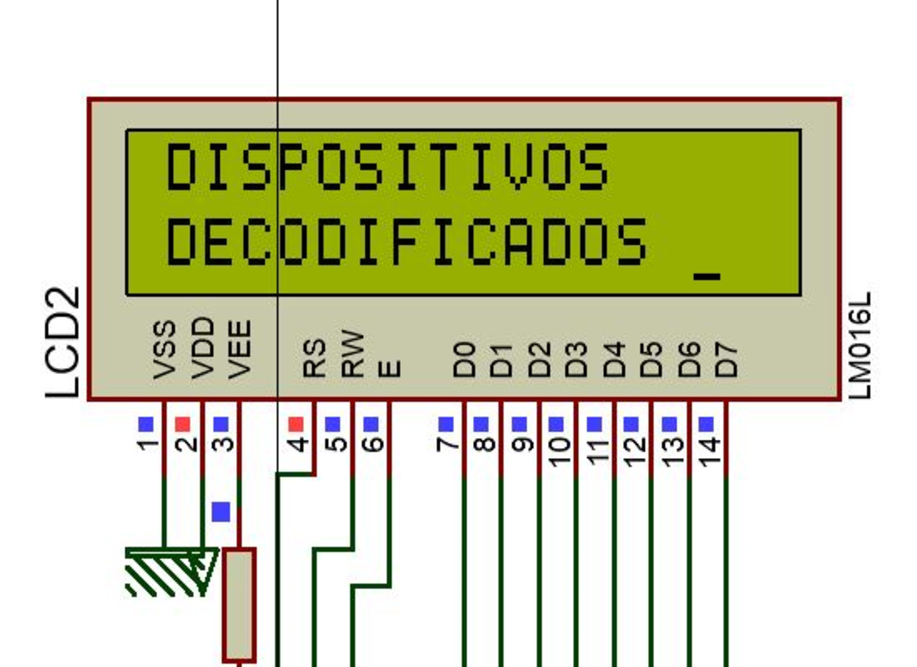
\includegraphics[width=.5\textwidth]{LCD.pdf}
\caption{Display LCD Funcionando No Porjeto de Dispositivos Decodificados}
\label{fig:adc_8051_dac_ideal}
\end{figure}

\begin{figure}[h!]
\centering
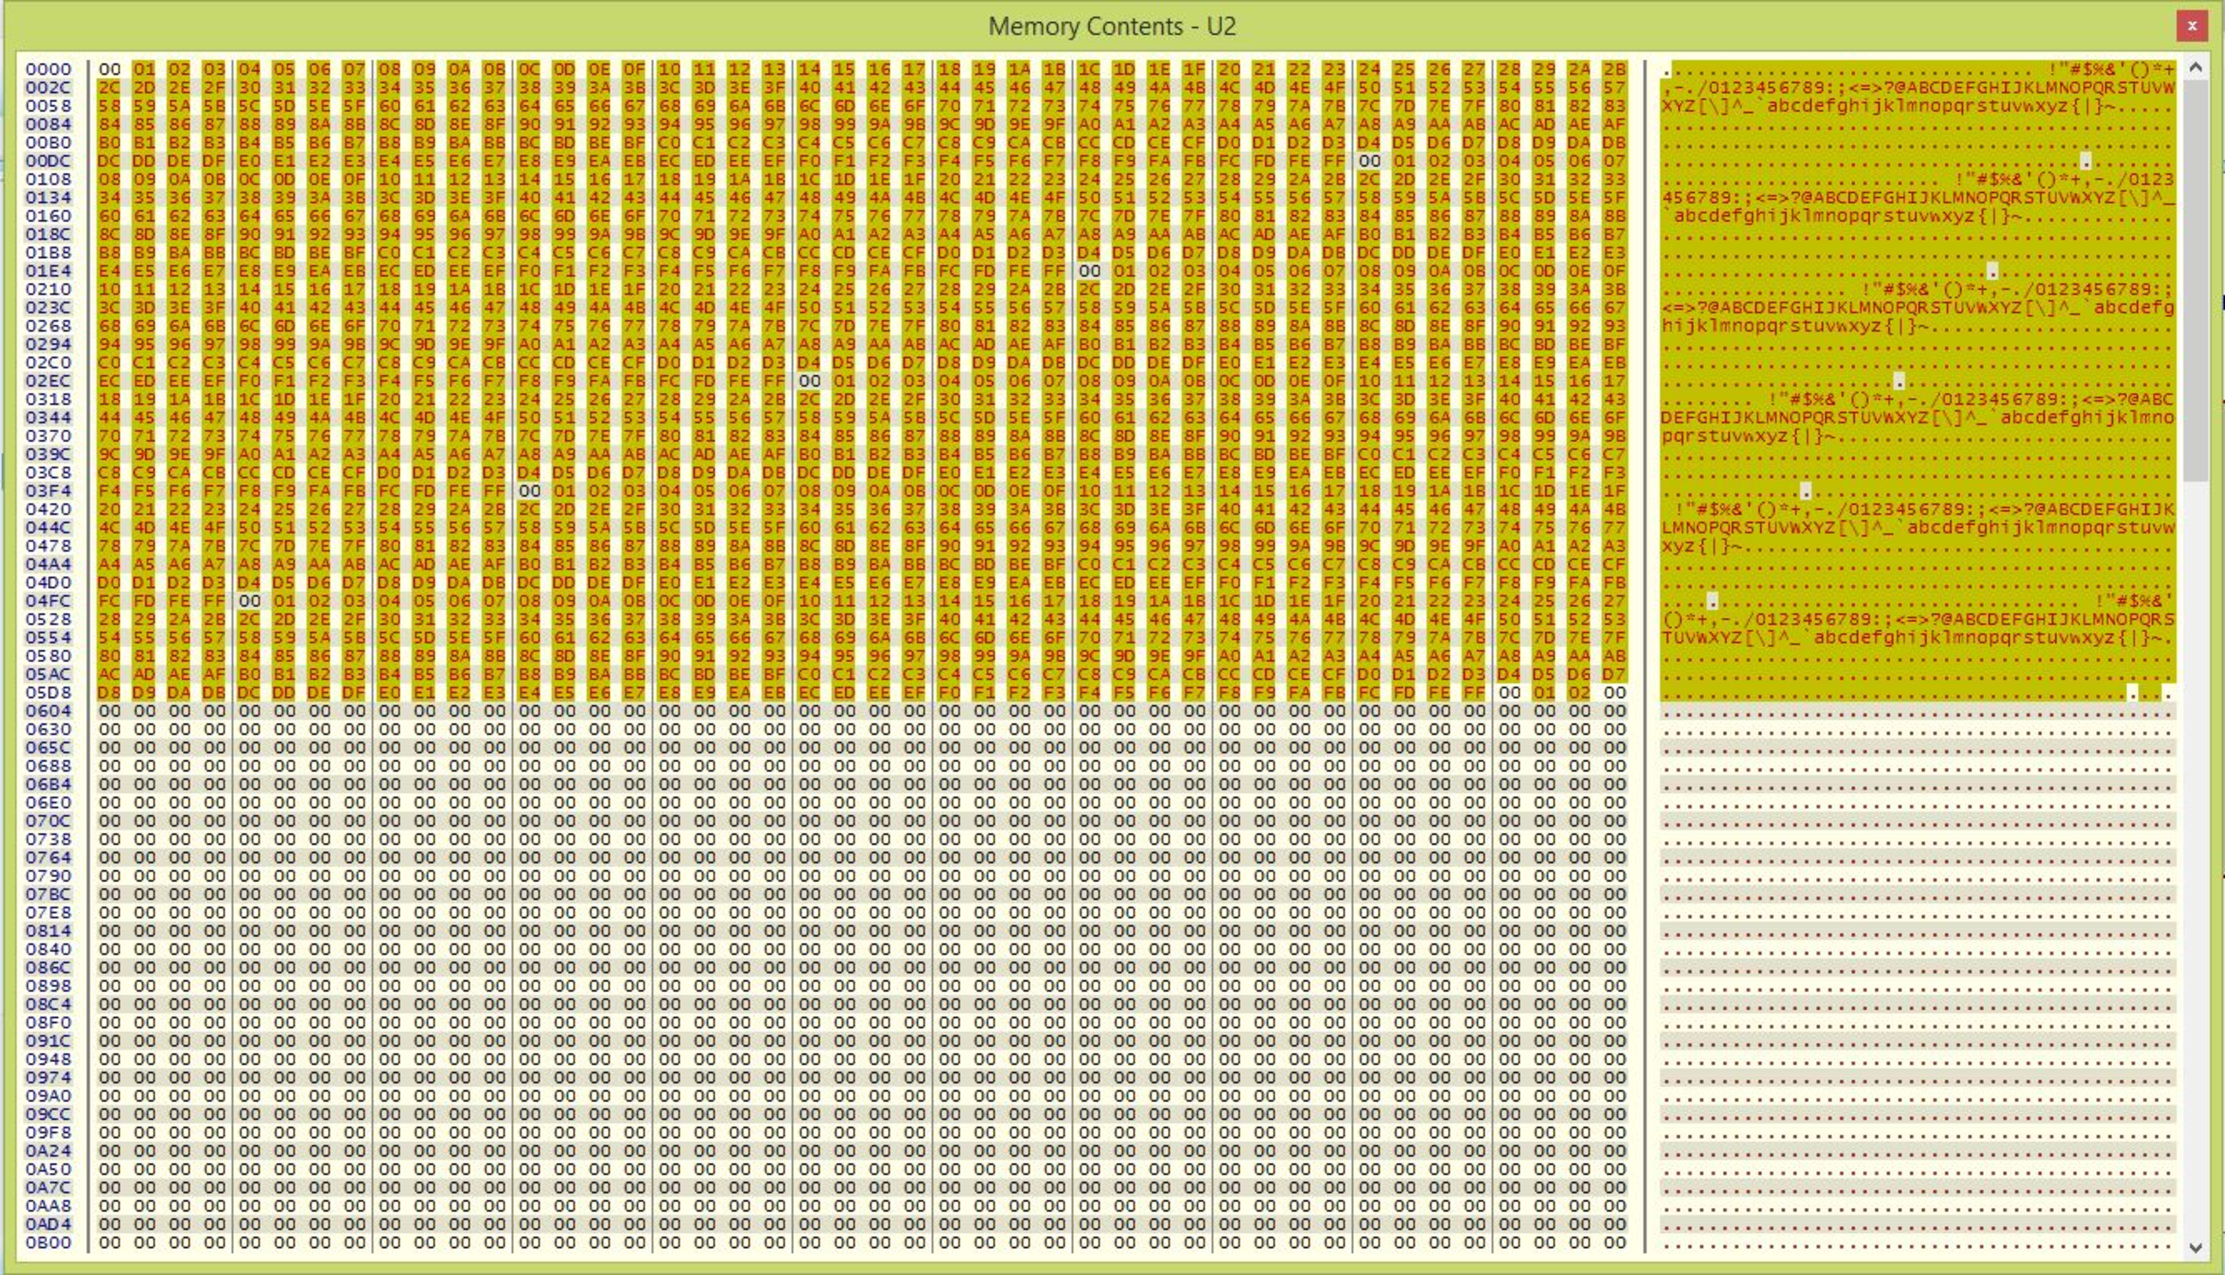
\includegraphics[width=.75\textwidth]{memory_contents.pdf}
\caption{Conteúdo da Memória Ram Após sua Utilização}
\label{fig:adc_8051_dac_ideal}
\end{figure}

\newpage

Abaixo encontra-se a placa resultante do projeto em questão.

\begin{figure}[h!]
\centering
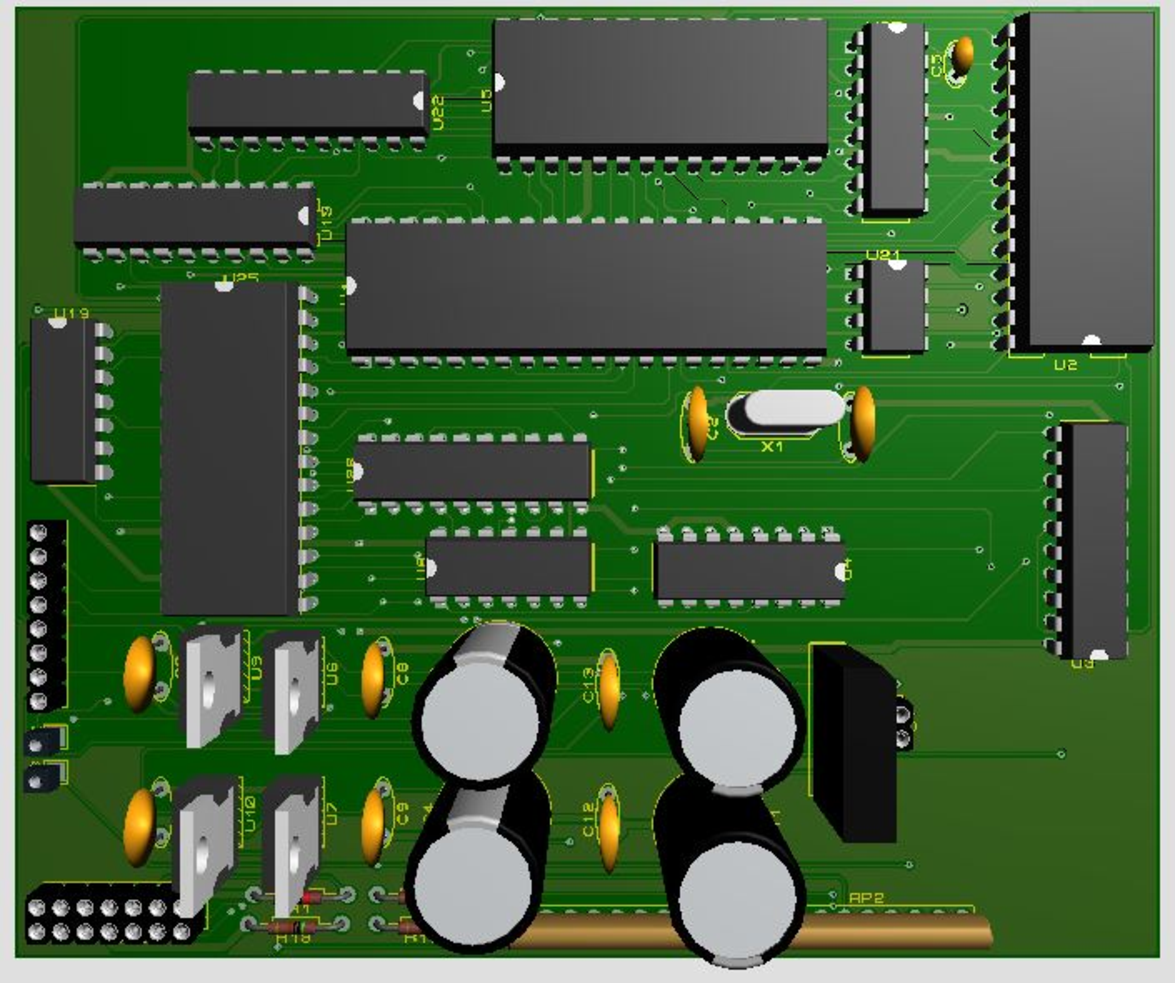
\includegraphics[width=1\textwidth]{Placa_Final.pdf}
\caption{Placa Renderizada do projeto em questão}
\label{fig:adc_8051_dac_ideal}
\end{figure}

\pagebreak

\section{Driver Do Motor de Passo}
A imagem com o esquemático do driver encontra-se abaixo e sua renderização em placa.

\begin{figure}[h!]
\centering
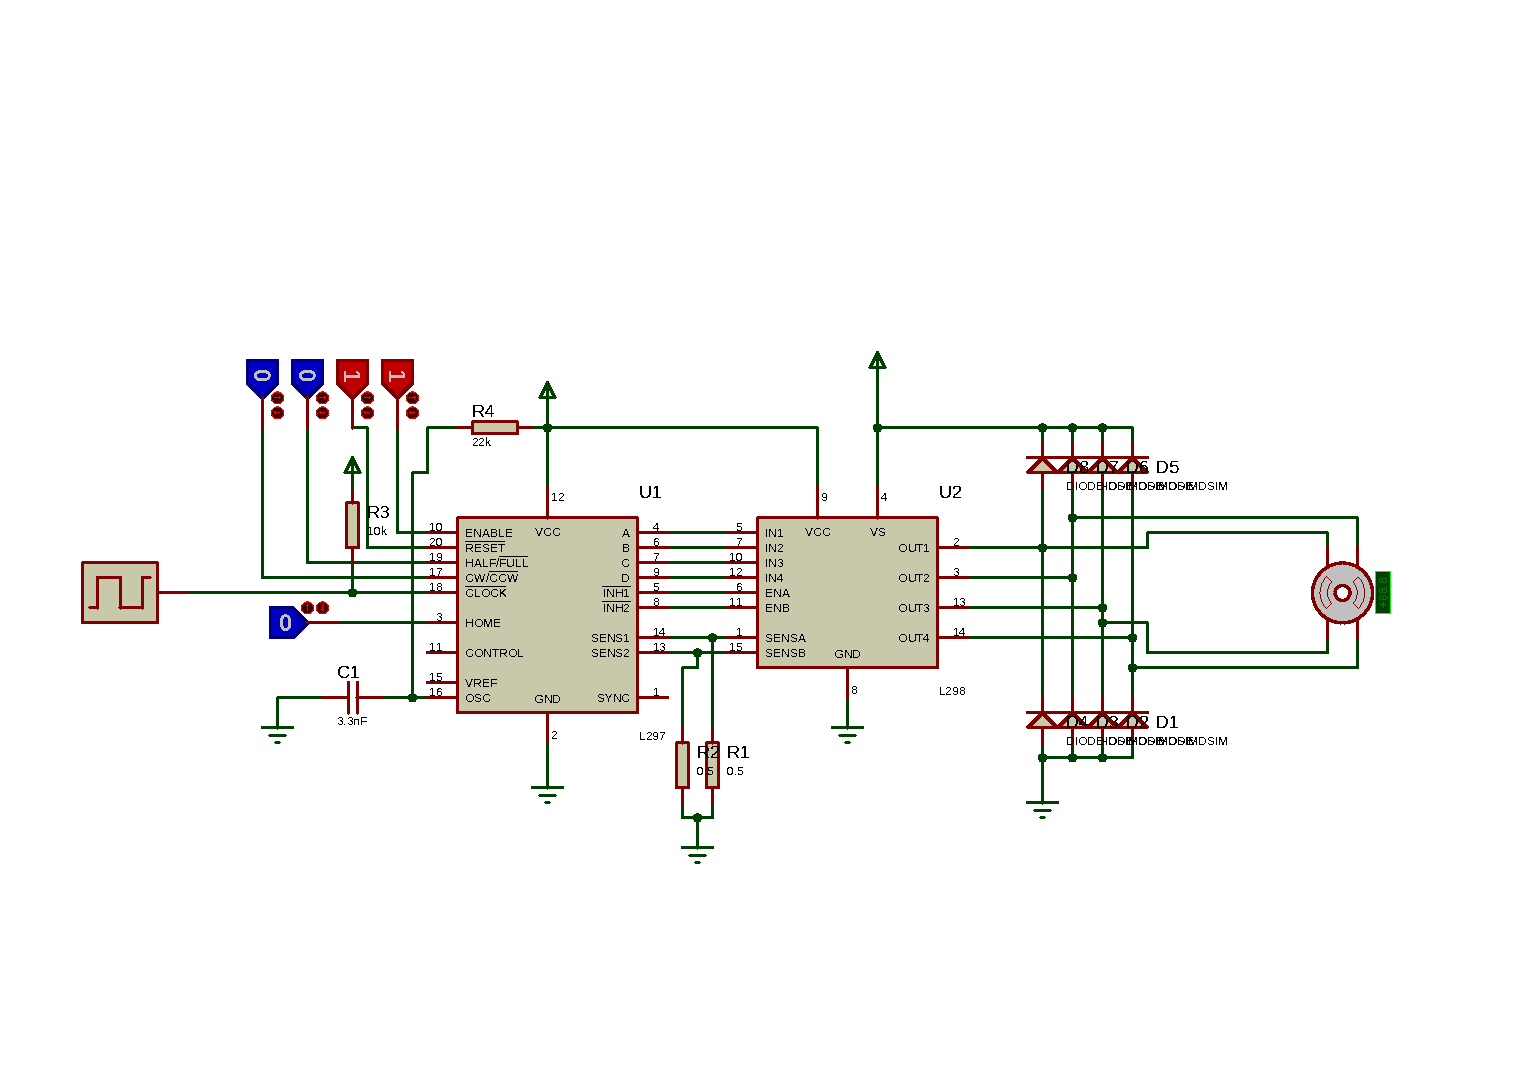
\includegraphics[width=.8\textwidth]{motor_driver.pdf}
\caption{Conteúdo da Memória Ram Após sua Utilização}
\label{fig:adc_8051_dac_ideal}
\end{figure}

\begin{figure}[h!]
\centering
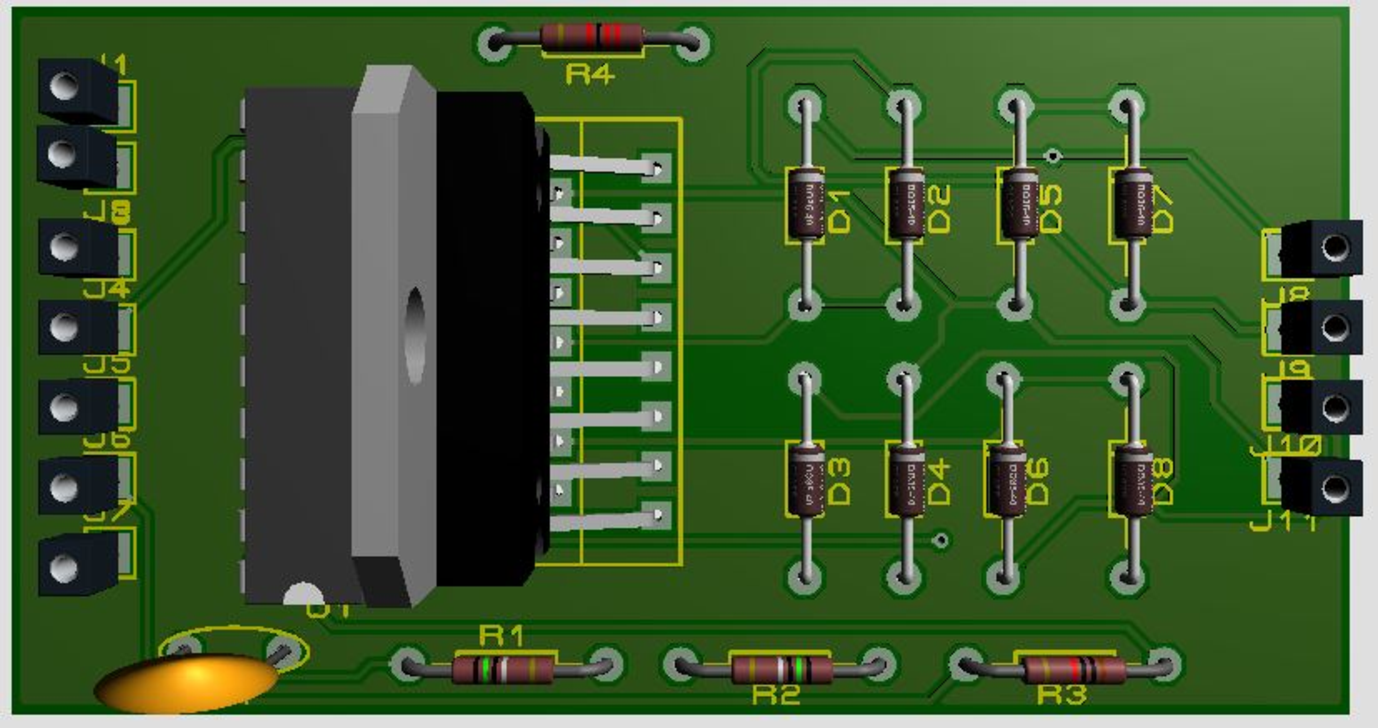
\includegraphics[width=.8\textwidth]{Motor_driver_renderizado.pdf}
\caption{Driver do motor de passo rendeirizado}
\label{fig:adc_8051_dac_ideal}
\end{figure}

\newpage

\section{Programas}
\subsection{Programa Conversor AD DA}
\begin{lstlisting}
 CLOCK  EQU P3.3;
START  EQU P3.4;
EOC    EQU P3.2;
 
	ORG 0000H;
	SJMP INICIO;

	ORG 0003H
	MOV A,P0;
	RETI;
	
	ORG 000BH;		INTERRUPÇÃO DO TIMER0 PARA O START DO ADC
	CPL CLOCK;
	LCALL INICIA_TIMER0;
	RETI;
			
INICIO:	MOV P0,#0FFH;
	SETB P2.7;
	CLR P2.6;
	CLR P2.5;
	CLR CLOCK;
	CLR START;
	LCALL INTERRUPTION_CONFIG;
	LCALL INICIA_TIMER0;
	;LCALL DELAY10US;
	LCALL PULSE;
LOOP:	
	CLR P2.7;
	CLR P2.6;
	CLR P2.5;
	MOV P0,#0FFH;
	JNB EOC,$;
	SETB P2.7;
	CLR P2.6;
	CLR P2.5;
		

	MOV A,P0;
	MOV P0,A;
	CLR P2.7;
	SETB P2.6;
	SETB P2.5;
	
	LCALL DELAY10US;
	LCALL PULSE;

	SJMP LOOP;

INTERRUPTION_CONFIG:
	SETB EA;
	;SETB EX0;
	SETB ET0;
	SETB PT0;
	MOV TCON,#11H;		
	RET;

INICIA_TIMER0:	
	MOV TH0,#0FFH;
	MOV TL0,#0FEH;
	SETB TR0;	
	RET;
	
DELAY10US:
	MOV	R0, #003h
	NOP
	DJNZ	R0, $
	NOP
	NOP
	RET;

PULSE:
	SETB START;
	MOV	R2, #002h
	MOV	R1, #087h
	MOV	R0, #00Fh
	NOP
	DJNZ	R0, $
	DJNZ	R1, $-5
	DJNZ	R2, $-9
	MOV	R0, #00Eh
	DJNZ	R0, $
	CLR START;
	RET;

	END;
\end{lstlisting}

\subsection{Programa Display LCD}
\begin{lstlisting}
RS EQU P2.0;
;RS=0 ENVIA INSTRUÇÕES PARA O DISPLAY
;RS=1 ENVIA DADOS A SEREM MOSTRADOS NO DISPLAY.
RW EQU P2.1;
;RW=0 PARA A ESCITA OU ENVIO DE INTRUÇÕES NO DISPLAY
;RW=1 PARA A LEITURA DE CARACTERES DO LCD
E  EQU P2.2;
;APÓS O DADO SER COLOCADO NO DUTO, TANTO PARA INSTRUÇÕES COMO ESCRITA DE CARACTERES, DEVE SER DADO UM PULSO DE ENABLE NO DISPLAY.
DADOS_INSTRUCOES EQU P0;
;FAZ UMA DIRETIVA NOMIAL PARA A PORTA AONDE ESTÁ LIGADO OS DADOS DO DISPLAY.

	ORG 0000H;
	CLR P2.5;
	SETB P2.6;
	CLR P2.7;
	LCALL INIT_LCD;
	MOV A,#00H;		ENDEREÇO DA PRIMEIRA POSIÇÃO DA PRIMEIRA LINHA.
	LCALL POS_LCD;
	MOV DPTR,#TAB1;
	LCALL ENVIA_FRASE;
	MOV A,#40H;		ENDEREÇO DA PRIMEIRA POSIÇÃO DA SEGUNDA LINHA.
	LCALL POS_LCD;
	MOV DPTR,#TAB2;
	LCALL ENVIA_FRASE;
	MOV P1,#00H;
	SJMP $;

INIT_LCD:
	MOV A,#32H;		NÃO SEI OQUE SIGNIFICA.(PESQUISAR)
	LCALL WRITEINSTRUCOES;
	MOV A,#28H;		MODO 2 LINHAS DE 4 BITS COM MASTRIZ 5/7 PONTOS.
	LCALL WRITEINSTRUCOES;
	MOV A,#0EH;		SEM CURSOR.
	LCALL WRITEINSTRUCOES;
	MOV A,#06H;		INCREMENTA O CURSOR A CADA ESCRITA DE DADOS.
	LCALL WRITEINSTRUCOES;
	MOV A ,#01H;		LIMPA O DISPLAYE RETORNA O CURSOR PARA O INICIO.
	LCALL WRITEINSTRUCOES;
	RET;

WRITEINSTRUCOES:
	SETB E;
	CLR RS;			MODO DE INTRUSÇÕES;
	CLR RW;			MODO DE ESCRITA DO LCD;
	MOV R7,A;
	ANL A,#0F0H;
	MOV DADOS_INSTRUCOES,A;
	CLR E;
	LCALL WAITLCD;
	SETB E;
	MOV A,R7;
	ANL A,#0FH;
	SWAP A;
	MOV DADOS_INSTRUCOES,A;
	CLR E;
	LCALL WAITLCD;
	SETB E;
	RET;

WRITEDADOS:
	SETB E;
	SETB RS;		MODO DE DADOS/CARACTERES;
	CLR RW;			MODO DE ESCRITA;
	MOV R7,A;
	ANL A,#0F0H;
	MOV DADOS_INSTRUCOES,A;
	CLR E;
	LCALL WAITLCD;
	SETB E;
	MOV A,R7;
	ANL A,#0FH;
	SWAP A;
	MOV DADOS_INSTRUCOES,A;
	CLR E;
	LCALL WAITLCD;	
	RET;

WAITLCD:
	MOV	R1, #006h
	MOV	R0, #0E4h
	NOP
	DJNZ	R0, $
	DJNZ	R1, $-5
	NOP
	NOP
	NOP
	NOP
	RET;	

POS_LCD:
	ADD A,#80H;		
	LCALL WRITEINSTRUCOES;
	RET;

ENVIA_FRASE:
	CLR A;
	MOVC A,@A+DPTR;
CONTINUA:
	LCALL WRITEDADOS;
	INC DPTR;
	CLR A;
	MOVC A,@A+DPTR;
	CJNE A,#'$',CONTINUA;
	RET;	

TAB1: 	DB 'ASSEMBLY 4 BITS $'
TAB2:	DB 'COM DUAS LINHAS $'
	END;
\end{lstlisting}

\begin{lstlisting}
	ORG 0000H;

	LCALL CONFIG_SERIAL;

COLUNA1:
	MOV P1,#00H;
	CLR P1.3;
	SETB P1.0;
ZERO:	
	JNB P1.4,UM;
	
	MOV DPTR,#TAB1;
	LCALL ENVIA_FRASE;
	MOV A,#00H;
	LCALL ENVIA_CARACTER;
	LCALL DELAY;
UM:
	JNB P1.5,DOIS;
	
	MOV DPTR,#TAB1;
	LCALL ENVIA_FRASE;
	MOV A,#01H;
	LCALL ENVIA_CARACTER;
	LCALL DELAY;
DOIS:
	JNB P1.6,TRES;

	MOV DPTR,#TAB1;
	LCALL ENVIA_FRASE;
	MOV A,#02H;
	LCALL ENVIA_CARACTER;
	LCALL DELAY;

TRES:	JNB P1.7,COLUNA2;

	MOV DPTR,#TAB1;
	LCALL ENVIA_FRASE;
	MOV A,#03H;
	LCALL ENVIA_CARACTER;
	LCALL DELAY;
	
COLUNA2:
	CLR P1.0;
	SETB P1.1;
QUATRO:

	JNB P1.4,CINCO;

	MOV DPTR,#TAB1;
	LCALL ENVIA_FRASE;
	MOV A,#04H;
	LCALL ENVIA_CARACTER;
	LCALL DELAY;

CINCO:
	JNB P1.4,SEIS;

	MOV DPTR,#TAB1;
	LCALL ENVIA_FRASE;
	MOV A,#05H;
	LCALL ENVIA_CARACTER;
	LCALL DELAY;

SEIS:
	JNB P1.6,SETE;

	MOV DPTR,#TAB1;
	LCALL ENVIA_FRASE;
	MOV A,#06H;
	LCALL ENVIA_CARACTER;
	LCALL DELAY;

SETE:
	JNB P1.7,COLUNA3;

	MOV DPTR,#TAB1;
	LCALL ENVIA_FRASE;
	MOV A,#07H;
	LCALL ENVIA_CARACTER;
	LCALL DELAY;
	

COLUNA3:
	CLR P1.1;
	SETB P1.2;
OITO:
	JNB P1.4,NOVE;

	MOV DPTR,#TAB1;
	LCALL ENVIA_FRASE;
	MOV A,#08H;
	LCALL ENVIA_CARACTER;
	LCALL DELAY;

NOVE:
	JNB P1.5,LETRA_A;

	MOV DPTR,#TAB1;
	LCALL ENVIA_FRASE;
	MOV A,#09H;
	LCALL ENVIA_CARACTER;
	LCALL DELAY;

LETRA_A:
	JNB P1.6,LETRA_B;

	MOV DPTR,#TAB1;
	LCALL ENVIA_FRASE;
	MOV A,#0AH;
	LCALL ENVIA_CARACTER;
	LCALL DELAY;

LETRA_B:
	JNB P1.7,COLUNA4;

	MOV DPTR,#TAB1;
	LCALL ENVIA_FRASE;
	MOV A,#0BH;
	LCALL ENVIA_CARACTER;
	LCALL DELAY;

COLUNA4:
	CLR P1.2;
	SETB P1.3;
LETRA_C:
	JNB P1.4,LETRA_D;

	MOV DPTR,#TAB1;
	LCALL ENVIA_FRASE;
	MOV A,#0CH;
	LCALL ENVIA_CARACTER;
	LCALL DELAY;

LETRA_D:
	JNB P1.5,LETRA_E;

	MOV DPTR,#TAB1;
	LCALL ENVIA_FRASE;
	MOV A,#0DH;
	LCALL ENVIA_CARACTER;
	LCALL DELAY;

LETRA_E:
	JNB P1.6,LETRA_F;

	MOV DPTR,#TAB1;
	LCALL ENVIA_FRASE;
	MOV A,#0EH;
	LCALL ENVIA_CARACTER;
	LCALL DELAY;

LETRA_F:
	JNB P1.7,FIM;

	MOV DPTR,#TAB1;
	LCALL ENVIA_FRASE;
	MOV A,#0FH;
	LCALL ENVIA_CARACTER;
	LCALL DELAY;

FIM:
	LJMP COLUNA1;
			
CONFIG_SERIAL:
	 MOV TMOD,#20H         ;TIMER 1 COMO TEMPORIZADOR DE 8 BITS AUTO-RECARREGÁVEL.  
	 MOV TH1,#253D         ;TH1 E TL1 CARREGADOS PARA BAUD RATE = 9600.  
	 MOV TL1,#253D  
	 MOV SCON,#01000000B   ;SERIAL MODO 1 (TAXA VARIÁVEL (10 BITS)) E RECEPÇÃO        				               ;DESABILITADA;  
	 SETB TR1              ;LIGA TIMER 1
	 RET;

CONVERTE_HEX_ASC:
	CJNE A,#0AH,TESTEA;
TESTEA: 
	JC NUM;
LETRA:	
	CLR C;
	ADD A,#37H;
	RET;
NUM:	
	CLR C;
	ADD A,#30H;
	RET;
	
ENVIA_FRASE:
	CLR A;
	MOVC A,@A+DPTR;
	MOV SBUF,A;
	JNB TI,$;
	CLR TI;
	INC DPTR;
	CLR A;
	MOVC A,@A+DPTR;			
	CJNE A,#'$',ENVIA_FRASE;
	RET;
	
ENVIA_CARACTER:
	MOV R1,A;
	ANL A,#0F0H;
	SWAP A;
	LCALL CONVERTE_HEX_ASC;
	MOV SBUF,A;
	JNB TI,$;
	CLR TI;
	LCALL SEGUNDO_CARACTER;
	RET;
			
SEGUNDO_CARACTER:
	MOV A,R1;
	ANL A,#0FH;
	LCALL CONVERTE_HEX_ASC;
	MOV SBUF,A;
	JNB TI,$;
	CLR TI;
	RET;

DELAY:
	MOV	R2, #01Ah
	MOV	R1, #0B1h
	MOV	R0, #017h
	NOP
	DJNZ	R0, $
	DJNZ	R1, $-5
	DJNZ	R2, $-9
	MOV	R0, #06Eh
	DJNZ	R0, $
	NOP
	RET;	
	
TAB1:   DB  0AH,0DH,'BOTAO PRESSIONADO = ','$';
	END;
	\end{lstlisting}
\subsection{Programa do prenchimento da memória ram}
	\begin{lstlisting}
	 	ORG 0000H;

	MOV DPTR,#0000H;
	MOV A,#00H;


RAM:	
	MOVX @DPTR,A;
	INC DPTR;
	INC A;
	SJMP RAM;
	END;

	\end{lstlisting}

\end{document}
